\documentclass{beamer}

% NOTE: reference
% https://arxiv.org/pdf/1604.05488.pdf

% HAGAR, first telescope to operate at an elevation > 4km
% http://www.tifr.res.in/~hagar/
% https://en.wikipedia.org/wiki/Indian_Astronomical_Observatory


\mode<presentation> {\usetheme{Madrid}}

\usepackage{graphicx}
\usepackage[utf8]{inputenc}
\usepackage{amsmath, amsthm, amssymb, mathtools}
\usepackage{hyperref}
\usepackage{flexisym}
\usepackage{mhchem}
\usepackage{textcomp}
\usepackage[export]{adjustbox}
\usepackage{subfig}
\graphicspath{{./img/}}

\title[TeV Astrophysics]{Astronomical facilities and instrumentation in TeV}

\author{Wei-Chih Huang}
\institute[NTHU]{
National Tsing Hua University \\
\medskip
}
\date{April 23, 2019}


\begin{document}


\begin{frame}{ICAT: H.E.S.S.}
	High Energy Stereoscopic System (H.E.S.S.)
	\newline
	28 m H.E.S.S. II telescope vs. 12 m H.E.S.S. I telescopes
	\begin{figure}[h]
		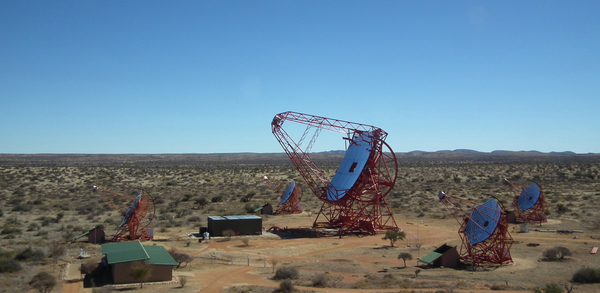
\includegraphics[width=280px]{Array_overviewS.jpg}
	\end{figure}
\end{frame}


\begin{frame}{ICAT: H.E.S.S.}
	Location: 23\textdegree16'18'' S, 16\textdegree30'00'' E at 1800 m
	\newline
	Detection method: Cherenkov technique
	\newline
	Target: gamma ray from Crab Nebula
	\begin{figure}[h]
		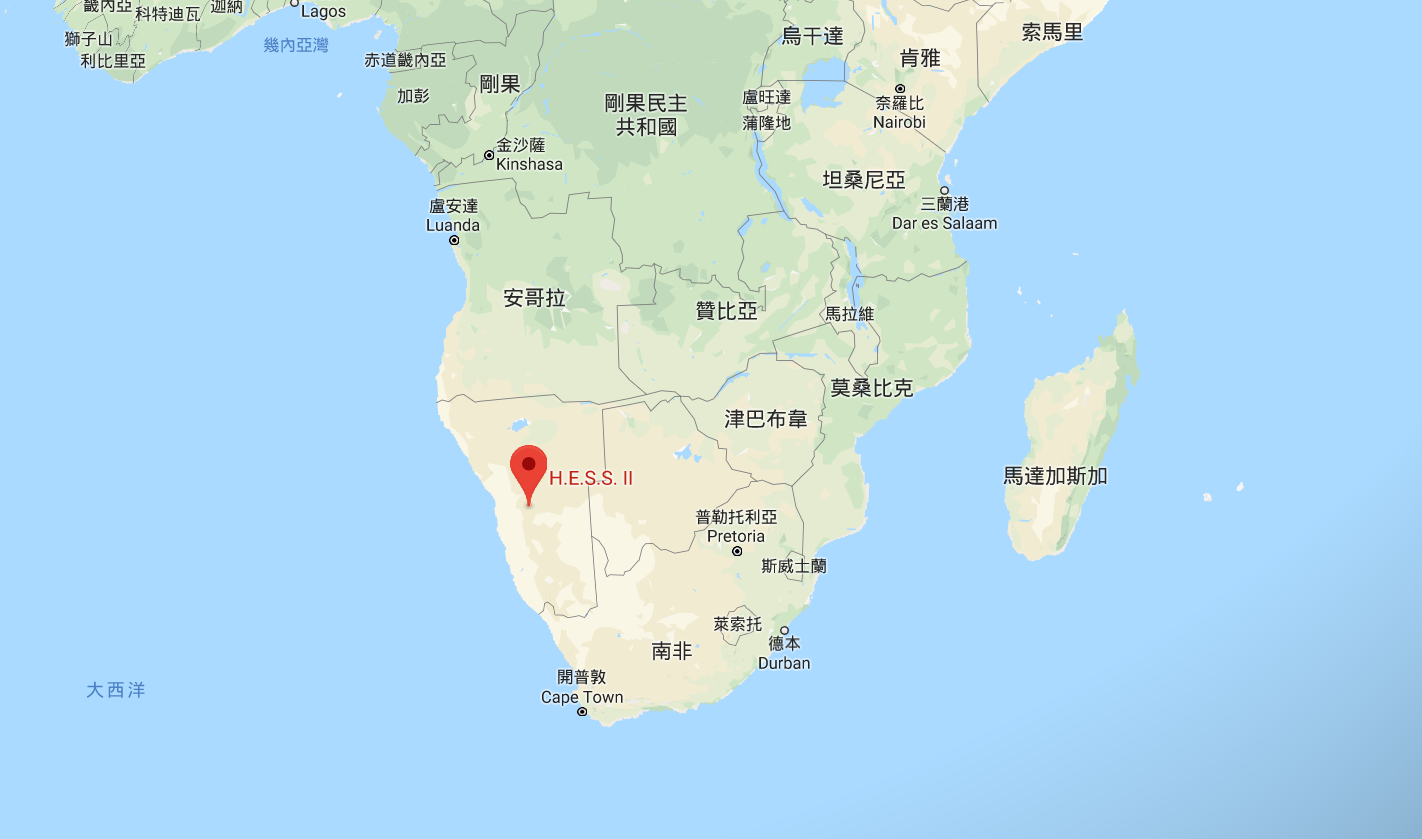
\includegraphics[width=280px]{HESS_location.png}
	\end{figure}
\end{frame}


\begin{frame}{ICAT: H.E.S.S.}
	The H.E.S.S. Collaboration
	\begin{itemize}
		\item 260 scientists
		\item 40 scientific institutions
		\item over 13 different countries
	\end{itemize}
	\begin{figure}[h]
		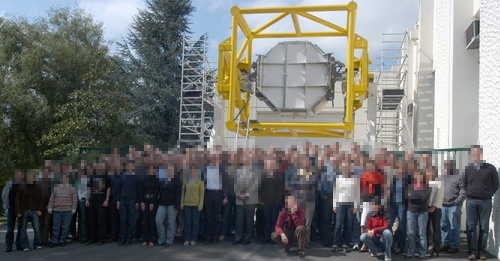
\includegraphics[width=280px]{hess_collaboration.jpg}
	\end{figure}
\end{frame}


\begin{frame}{ICAT: H.E.S.S.}
	Brief history:
	\begin{enumerate}
		\item summer 2002, first operation
		\item Sep 28, 2004, officially inaugurated
		\item 2006, ranked as the 10th most influential observatory worldwide
		\item July 2012, A much larger fifth telescope - H.E.S.S. II installed
		\item Sept. 30, 2012, open day for giant new H.E.S.S. II telescope
		\item 2015-2016, cameras full refurbished
		\item Sep. 27th, 2016, new camera inaugurated
	\end{enumerate}
	\begin{figure}[h]
		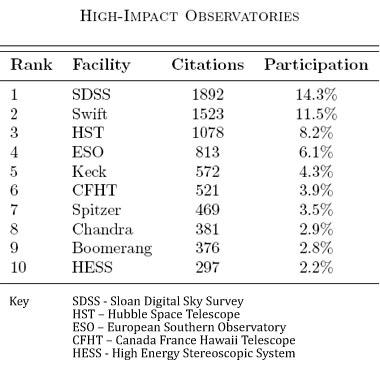
\includegraphics[width=120px]{telescopes-rank.jpg}
	\end{figure}
\end{frame}



\begin{frame}{ICAT: H.E.S.S. telescope}
	Azimuth drive system:
	\begin{itemize}
		\item 12 wheels in 6 bogies on 36 m diameter rail
		\item 4 wheels driven by motors
		\item peak positioning speed 200 degree/minute
		\item range $\pm$ 280 degree
	\end{itemize}
	\hfill \break
	Elevation drive system:
	\begin{itemize}
		\item height of elevation axis: 24 m
		\item 2 drive units with 2 motors each
		\item peak positioning speed 100 degree/minute
		\item range –125 degree +90 degree from vertical
	\end{itemize}
	\hfill \break
	Dish dimensions 32.6 m by 24.3 m ( $\approx$ 28 m circular dish.)
\end{frame}

\begin{frame}{ICAT: H.E.S.S. telescope}
	Elevation drive system
	\, \, \, (the VIDEO)
	\begin{figure}[h]
		\includegraphics[width=280px]{Elevation_Drive_1.JPG}
	\end{figure}
\end{frame}

\begin{frame}{ICAT: H.E.S.S. mirror}
	28 m H.E.S.S. II mirror:
	\begin{itemize}
		\item parabolic shape
		\item Focal length: 36 m
		\item Total mirror area: 614 $m^2$
	\end{itemize}
	\hfill \break
	Mirror facets:
	\begin{itemize}
		\item 875 hexagonal facets of 90 cm (flat-to-flat) size
		\item quartz-coated aluminized glass
		\item weight: 25 kg per facet approx
	\end{itemize}
\end{frame}

\begin{frame}{ICAT: H.E.S.S. mirror}
	Facet alignment: each facet is equipped with 2 actuators with 2 $\mu\text{m}$ positioning step size, corresponding to a 1 arc second facet tilt.
	\begin{figure}[h]
		\includegraphics[width=280px]{2012_mirrors.JPG}
	\end{figure}
\end{frame}


\begin{frame}{ICAT: H.E.S.S. camera}
	The camera of the 28 m telescope:
	\begin{itemize}
		\item Photo sensors: 2048 1-1/4’ photo multipliers
		\item Pixel size: 42 mm (hexagonal, flat-to-flat) $\approx$ 0.067 degree
		\item Sensitive area/field of view: 3.2 degree on the sky
		\item Signal recording: 1 GHz signal sampling; 2 gain channels or each pixel for large dynamic range; records signal amplitude, timing, and shape
		\item Effective signal integration time: 16 ns
		\item Image recording rate: 3600 images/second
		\item Power consumption: 8 kW
		\item Dimensions of camera body: 2.27 wide x 2.4 high x 1.84 deep (meter)
		\item Camera weight: 2.8 tons
		\item Camera support: Quadrupod
	\end{itemize}
\end{frame}


\end{document}